\documentclass[11pt,a4paper]{article}

% 1. Importar configuración y paquetes
\usepackage{packages}

\begin{document}

% 2. Insertar la portada
\begin{titlepage}
    \centering
    \vspace*{0.5cm}
    
    
\includegraphics[width=0.75\textwidth]{Images/LogoUps.png}
    \vspace{0.8cm}
    
    {\fontsize{16}{20}\selectfont\textbf{UNIVERSIDAD POLITÉCNICA SALESIANA}}\\[0.4cm]
    {\large\textbf{Área de Conocimiento: Ciencia y Tecnología}}\\[0.2cm]
    {\large\textbf{Carrera de Computación}}\\[1.2cm]
    
    \textcolor{upsblue}{\rule{\linewidth}{2pt}}\\[0.5cm]
    {\fontsize{18}{22}\selectfont\textbf{INFORME DE IMPLEMENTACIÓN DE SISTEMA}}\\[0.4cm]
    {\large\textbf{Caso de Estudio: Tienda de Venta de Comida de Mascotas}}\\[0.2cm]
    {\normalsize\textit{``PetShop Huellitas \& Snacks''}}\\[0.4cm]
    \textcolor{upsblue}{\rule{\linewidth}{2pt}}\\[1.5cm]
    
    \vfill
    
    \begin{flushright}
        \begin{minipage}{0.65\textwidth}
            \small
            \renewcommand{\arraystretch}{1.2}
            \begin{tabular}{r l}
                \textbf{Integrantes:} & 1. Daniel Guanga \\
                                      & 2. Leo Vasconez \\
                                      & 3. Xavier Siguachi \\[0.15cm]
                \textbf{Docente:}     & Ing. Diana Arce Cuesta \\
                \textbf{Asignatura:}  & Análisis y Diseño de Sistemas \\
                \textbf{Fecha:}       & \today
            \end{tabular}
        \end{minipage}
    \end{flushright}
    
    \vspace{1cm}
\end{titlepage}

\newpage
\tableofcontents
\newpage

% 3. Insertar el contenido por secciones
% (Debes crear estos archivos dentro de la carpeta Sections/)
\section{Introducción y Objetivos}

\subsection{Introducción}
El sector comercial de productos y alimentos balanceados para mascotas en el Ecuador ha experimentado un crecimiento acelerado en los últimos años, impulsado por una mayor concientización sobre el bienestar animal y la tenencia responsable. Sin embargo, establecimientos comerciales de tamaño mediano como ``PetShop Huellitas \& Snacks'' se enfrentan a desafíos significativos al gestionar sus existencias y canales de atención de manera tradicional y manual. La falta de automatización y de sincronía entre el almacén físico y las solicitudes de pedidos genera ineficiencias operativas y constantes quiebres de stock. 

Ante este escenario, la implementación de un sistema de software enfocado a la automatización de procesos operativos se presenta como una solución fundamental para optimizar la cadena de valor del negocio y garantizar su supervivencia frente al ingreso de competidores de gran escala. Este informe presenta el análisis y diseño detallado de la solución informática denominada ``PetFood-Manager'', estructurando sus requerimientos, diagramas de interacción y diagramas estructurales para fundamentar un desarrollo de software robusto, transaccional y escalable.

\subsection{Objetivos del Proyecto}

\subsubsection{Objetivo General}
Diseñar el modelo de sistema informático ``PetFood-Manager'' para la tienda de venta de comida de mascotas ``PetShop Huellitas \& Snacks'', con el fin de automatizar el control de inventario en tiempo real, agilizar el procesamiento de pedidos de clientes y sistematizar el reabastecimiento con los proveedores bajo una estrategia de supervivencia eficiente.

\subsubsection{Objetivos Específicos}
\begin{itemize}
    \item Contextualizar el flujo de información de la tienda mediante el modelado del diagrama de contexto y el diagrama de flujo de datos (DFD) de nivel 0, delimitando claramente las interacciones con clientes, proveedores y entes externos.
    \item Modelar el comportamiento dinámico y la estructura de clases del sistema utilizando la notación UML, detallando la interacción lógica de los componentes de software mediante diagramas de secuencia, actividades y clases.
    \item Definir la arquitectura física y de componentes del sistema considerando un despliegue distribuido en la nube, garantizando requerimientos no funcionales de seguridad, integridad y alta disponibilidad de la información.
\end{itemize}
\section{Datos Generales y gestión estratégica}

\subsection{Nombre de la empresa. Dirección}
\textbf{Nombre Comercial:} PetShop Huellitas \& Snacks \\
\textbf{Dirección Física:} Av. de los Granados N34-12 y Av. 6 de Diciembre, Edificio Plaza Norte, Planta Baja, Quito, Ecuador.

\subsection{Descripción de las actividades}
PetShop Huellitas \& Snacks es un establecimiento minorista dedicado a la comercialización de comida balanceada, galletas, snacks orgánicos y suplementos nutricionales para mascotas domésticas (perros, gatos, aves y roedores). Las actividades principales de la empresa incluyen el abastecimiento con distribuidores nacionales e importadores, la gestión física del inventario del local, la venta directa en el establecimiento físico, y la distribución de pedidos a domicilio a través de su canal de delivery rápido para el sector norte y centro de la ciudad de Quito.

\subsection{Foto de la empresa}
\begin{figure}[H]
    \centering
    % Asegúrate de que esta imagen exista en tu carpeta Images/
    
\includegraphics[width=0.70\textwidth]{Images/FotoTienda.png}
    \caption{Fachada del establecimiento de la Tienda de Comida de Mascotas}
    \label{fig:foto_empresa}
\end{figure}

\subsection{Análisis FODA}
\begin{table}[H]
    \centering
    \small
    \renewcommand{\arraystretch}{1.4}
    \begin{tabularx}{\textwidth}{|X|X|}
        \hline
        \rowcolor{upsblue} \multicolumn{2}{|c|}{\textcolor{white}{\textbf{MATRIZ FODA}}} \\
        \hline
        \rowcolor{lightgray} \textbf{Fortalezas (F)} & \textbf{Debilidades (D)} \\
        \hline
        1. Stock diverso y constante de marcas premium de alimento (Royal Canin, Hills, ProPlan) y snacks especializados. \par
        2. Servicio a domicilio establecido y consolidado en el norte y centro de la ciudad. & 
        1. Registro lento de pedidos de clientes realizados de forma manual mediante WhatsApp y canales de voz. \par
        2. Falta de consistencia e integración inmediata entre el stock físico disponible y el stock lógico registrado. \\
        \hline
        \rowcolor{lightgray} \textbf{Oportunidades (O)} & \textbf{Amenazas (A)} \\
        \hline
        1. Aumento del número de hogares de la zona con mascotas que requieren compras de alimento mensuales. \par
        2. Disposición del usuario a suscribirse a portales de envíos recurrentes programados. & 
        1. Competencia directa de supermercados de gran escala que ofertan marcas estándar a bajo costo. \par
        2. Demoras y problemas logísticos por parte de importadores mayoristas de productos premium. \\
        \hline
    \end{tabularx}
    \caption{Análisis FODA - PetShop Huellitas \& Snacks}
    \label{tab:foda}
\end{table}

\subsection{Estrategia de Supervivencia MIN-MIN}\label{sec:estrategia}
Tras el análisis de los factores de la matriz FODA, se determinó que el proyecto debe guiarse por la \textbf{Estrategia de Supervivencia (MIN-MIN)} para contrarrestar las debilidades internas y resistir a las amenazas externas. 

El cruce de factores se realiza vinculando las debilidades de registro manual de pedidos y desorganización de inventario (D1, D2) con la amenaza de grandes supermercados competidores directos (A1). Para competir y subsistir, PetShop Huellitas \& Snacks requiere implementar el sistema informático transaccional ``PetFood-Manager'' que automatice el inventario y controle el stock en tiempo real. Al suprimir errores de stock y acelerar los pedidos mediante una pasarela web ágil, el negocio optimiza sus costos operativos y previene retrasos de abastecimiento, permitiéndole mantener la fidelidad de sus clientes y asegurar su rentabilidad frente al retail masivo.

A continuación, se detalla la matriz de cruce para la formulación de las estrategias de supervivencia (MIN-MIN) en función de las amenazas externas identificadas:

\begin{table}[H]
    \centering
    \small
    \renewcommand{\arraystretch}{1.4}
    \begin{tabularx}{\textwidth}{|L|p{4cm}|L|}
        \hline
        \rowcolor{upsblue}
        \textcolor{white}{\textbf{Amenaza (Entorno)}} & 
        \textcolor{white}{\textbf{Debilidad Interna}} & 
        \textcolor{white}{\textbf{Estrategia de Supervivencia (MIN-MIN)}} \\
        \hline
        \textbf{A1: Competencia directa de supermercados de gran escala} con marcas genéricas de bajo costo. & 
        \textbf{D1:} Registro manual e ineficiente de pedidos. \par
        \textbf{D2:} Desvinculación de stock físico y lógico. & 
        \textbf{Estrategia DA1 (Sincronización Transaccional):} Implementar la pasarela de pedidos y catálogo web en el sistema ``PetFood-Manager'' enlazado en tiempo real al inventario. Al acelerar la facturación y el delivery propio, se retiene a los clientes mediante excelencia en servicio frente al retail masivo. \\
        \hline
        \textbf{A2: Demoras logísticas de importadores} en abastecer marcas premium. & 
        \textbf{D2:} Falta de control preventivo de existencias. & 
        \textbf{Estrategia DA2 (Alertas Tempranas):} Configurar límites de stock mínimo por alimento en el catálogo que disparen alertas automáticas de compra al proveedor. Esto permite realizar pedidos con anticipación, previniendo quiebres de stock ante demoras de importación. \\
        \hline
    \end{tabularx}
    \caption{Matriz de Estrategias de Supervivencia MIN-MIN por Amenazas}
    \label{tab:estrategias_minmin}
\end{table}
\section{Información del entorno}

\subsection{Descripción del entorno}
El entorno operativo de PetShop Huellitas \& Snacks está conformado por los siguientes actores clave:
\begin{itemize}
    \item \textbf{Proveedores:} Distribuidoras mayoristas de alimentos premium nacionales y extranjeras, y fabricantes de accesorios y snacks.
    \item \textbf{Clientes:} Propietarios de mascotas domésticas, albergues de rescate animal y clínicas veterinarias minoristas del norte de Quito.
    \item \textbf{Competencia:} Grandes supermercados locales, almacenes agropecuarios y otras tiendas online que comercializan alimento para mascotas.
    \item \textbf{Estado:} El Servicio de Rentas Internas (SRI) que norma la emisión de facturación electrónica y entidades de control de registros sanitarios.
    \item \textbf{Comunidad:} Fundaciones locales de protección de mascotas, dueños de mascotas de la zona residencial y vecinos del local.
\end{itemize}

\subsection{Entidades}
\begin{enumerate}
    \item \textbf{Cliente (Actor Externo):} Interactúa con el sistema para consultar productos, realizar compras y recibir notificaciones y comprobantes electrónicos.
    \item \textbf{Administrador / Vendedor (Actor Interno):} Administra el catálogo de productos, visualiza reportes de stock, aprueba pedidos y despacha compras.
    \item \textbf{Proveedor (Actor Externo):} Sistema o persona que recibe solicitudes automáticas de reabastecimiento generadas por el sistema.
    \item \textbf{Pasarela de Pagos (Sistema Externo):} Entidad bancaria o pasarela transaccional externa encargada de validar los pagos electrónicos de los pedidos.
    \item \textbf{Facturación SRI (Sistema Externo):} Servicio del Estado que valida, autoriza y firma la emisión de comprobantes electrónicos del local.
\end{enumerate}

\subsection{Modelo de Contexto}
El diagrama de contexto define la frontera del sistema ``PetFood-Manager'', determinando los flujos de datos entrantes y salientes entre la aplicación central y las entidades externas definidas previamente.
\begin{figure}[H]
    \centering
    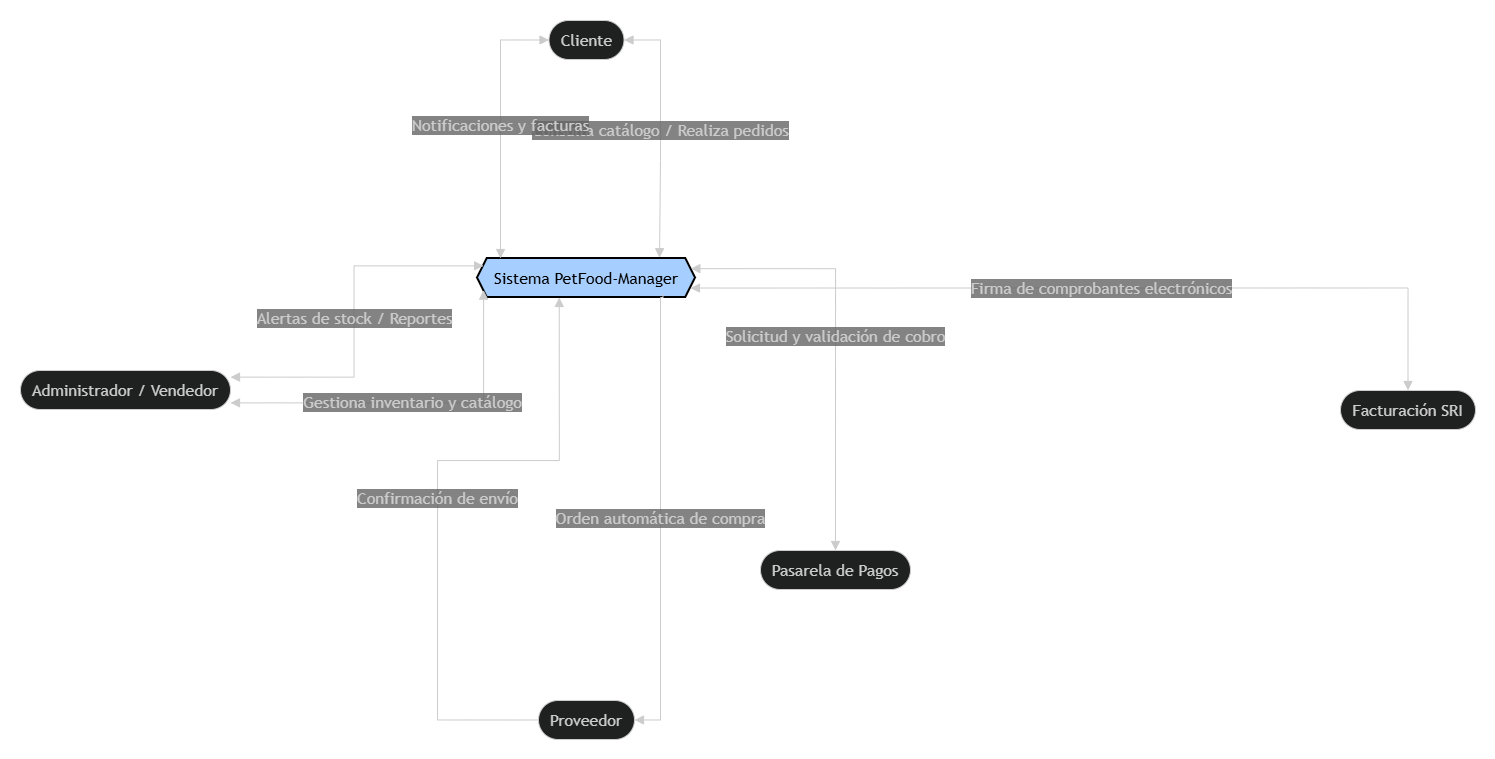
\includegraphics[width=0.60\textwidth]{Images/modeloContexto.png}
    \caption{Diagrama de Modelo de Contexto}
    \label{fig:modelo_contexto}
\end{figure}

\subsection{Diagrama de Flujo de Datos Nivel 0}
El DFD Nivel 0 subdivide el comportamiento del sistema en tres procesos transaccionales centrales que interactúan de forma directa con los almacenes de datos de la tienda.
\begin{figure}[H]
    \centering
    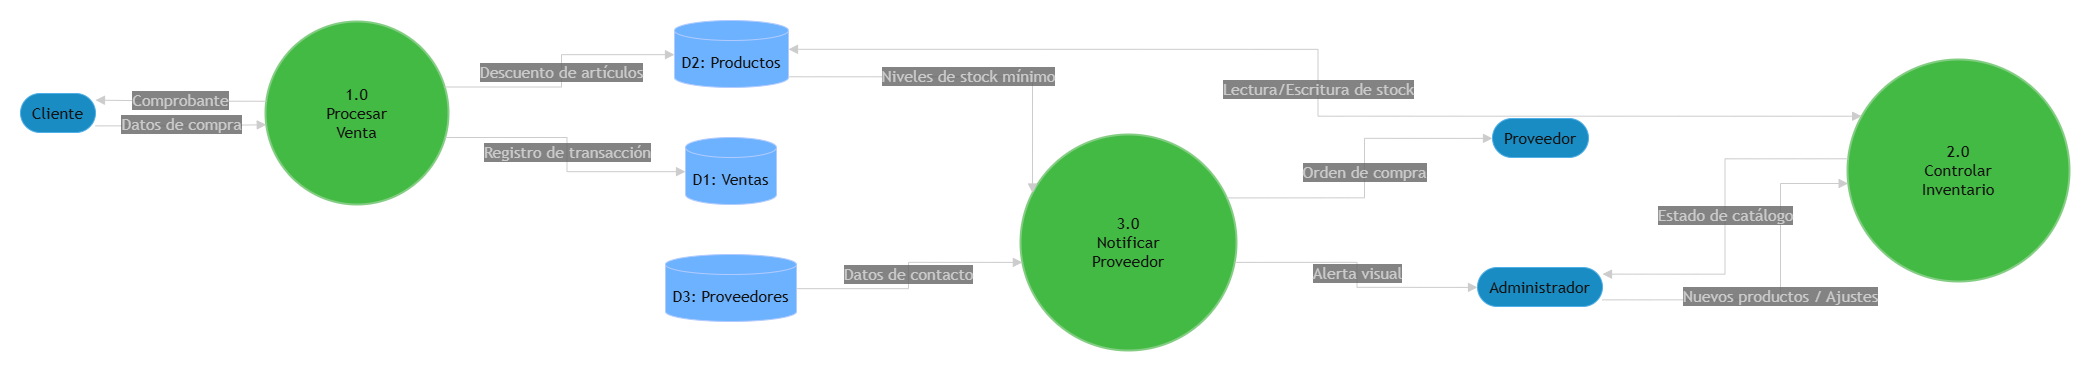
\includegraphics[width=0.60\textwidth]{Images/diagramaFlujo.png}
    \caption{Diagrama de Flujo de Datos (DFD) Nivel 0}
    \label{fig:dfd_nivel_0}
\end{figure}
\section{Requerimientos del Sistema}

\subsection{Definición del sistema informático basado en la estrategia de supervivencia MIN-MIN}
El sistema propuesto, ``PetFood-Manager'', se fundamenta en la estrategia de supervivencia MIN-MIN definida en la sección \ref{sec:estrategia}. Su propósito es reducir el procesamiento manual e ineficiente de pedidos y la desvinculación de inventarios frente a la amenaza de las grandes cadenas comerciales, automatizando el control de existencias en tiempo real y optimizando el reabastecimiento con los proveedores para asegurar la continuidad y competitividad del negocio.

\subsection{Listado de requerimientos funcionales}
\begin{table}[H]
    \centering
    \small
    \renewcommand{\arraystretch}{1.4}
    \begin{tabularx}{\textwidth}{|l|p{4.5cm}|L|}
        \hline
        \rowcolor{upsblue} \textcolor{white}{\textbf{ID}} & \textcolor{white}{\textbf{Requerimiento Funcional}} & \textcolor{white}{\textbf{Descripción / Detalle}} \\
        \hline
        \textbf{RF-01} & Registro de Catálogo de Alimentos & El sistema permitirá al Administrador registrar nuevos alimentos detallando marca, tipo de mascota (perro/gato), peso neto (kg), stock disponible, stock mínimo y costo unitario. \\
        \hline
        \textbf{RF-02} & Carrito de Compras y Pagos & El sistema permitirá a los clientes seleccionar productos del inventario disponible, agregarlos al carro de compras y pagar mediante pasarela de pagos integrada. \\
        \hline
        \textbf{RF-03} & Alertas y Órdenes Automáticas & El sistema enviará una alerta visual al Administrador y una orden de compra automática al Proveedor asignado cuando las existencias desciendan de su stock mínimo configurado. \\
        \hline
    \end{tabularx}
    \caption{Tabla de Requerimientos Funcionales}
    \label{tab:requerimientos_funcionales}
\end{table}

\subsection{Listado de requerimientos no funcionales}
\begin{table}[H]
    \centering
    \small
    \renewcommand{\arraystretch}{1.4}
    \begin{tabularx}{\textwidth}{|l|p{4.5cm}|L|}
        \hline
        \rowcolor{upsblue} \textcolor{white}{\textbf{ID}} & \textcolor{white}{\textbf{Requerimiento No Funcional}} & \textcolor{white}{\textbf{Descripción / Criterio de Medición}} \\
        \hline
        \textbf{RNF-01} & Tiempo de Respuesta & El sistema debe recuperar el estado del catálogo y la disponibilidad de stock en menos de 1.5 segundos ante consultas concurrentes de hasta 100 usuarios. \\
        \hline
        \textbf{RNF-02} & Seguridad de Información & Toda la información de transacciones y datos de tarjeta de crédito debe viajar encriptada mediante protocolo SSL/TLS con HTTPS activo en el dominio. \\
        \hline
        \textbf{RNF-03} & Alta Disponibilidad & Los servicios backend de API y base de datos relacional deben mantener una disponibilidad mínima anual del 99.9\% alojados sobre infraestructura de Azure. \\
        \hline
    \end{tabularx}
    \caption{Tabla de Requerimientos No Funcionales}
    \label{tab:requerimientos_no_funcionales}
\end{table}
\section{Casos de uso}

\subsection{Diagramas de casos de uso}
\begin{figure}[H]
    \centering
    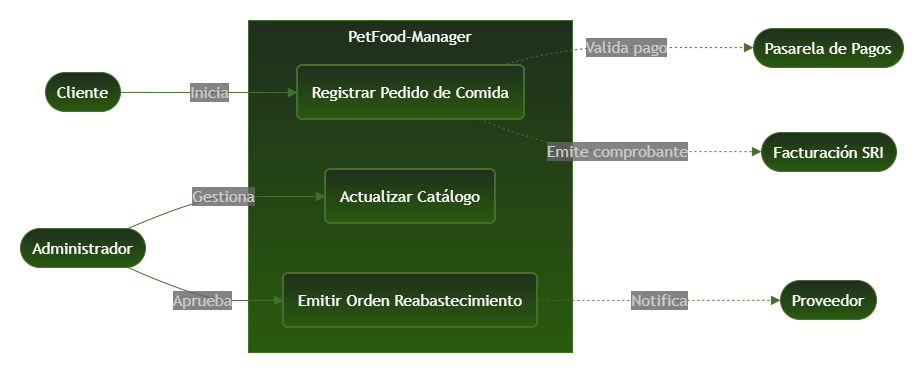
\includegraphics[width=0.60\textwidth]{Images/diagramaCasosUsos.png}
    \caption{Diagrama de Casos de Uso General}
    \label{fig:cu_general}
\end{figure}

\begin{figure}[H]
    \centering
    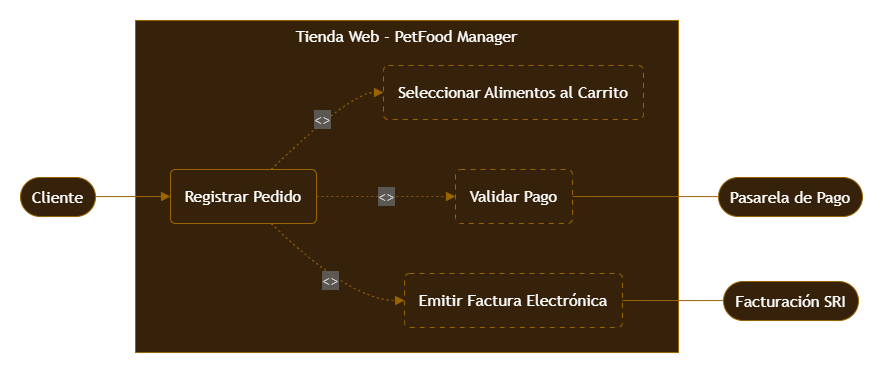
\includegraphics[width=0.60\textwidth]{Images/registroPedidoClase.png}
    \caption{Diagrama de Caso de Uso Específico 1}
    \label{fig:cu_especifico_1}
\end{figure}

\begin{figure}[H]
    \centering
    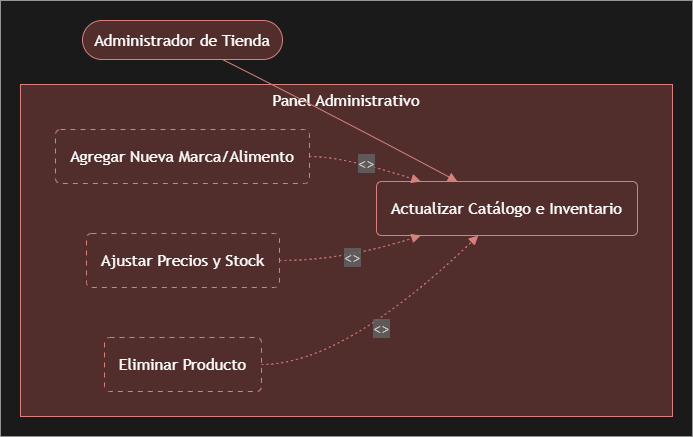
\includegraphics[width=0.60\textwidth]{Images/actualizarCatalogoClase.png}
    \caption{Diagrama de Caso de Uso Específico 2}
    \label{fig:cu_especifico_2}
\end{figure}

\begin{figure}[H]
    \centering
    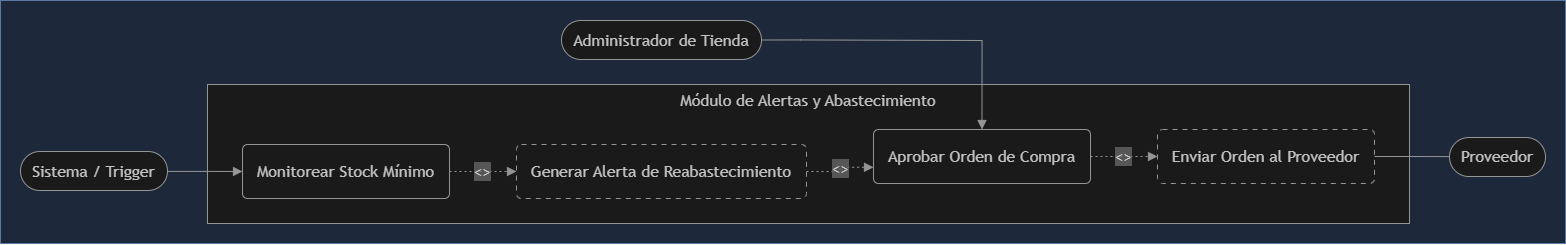
\includegraphics[width=0.60\textwidth]{Images/alertaRebstecimientoClase.png}
    \caption{Diagrama de Caso de Uso Específico 3}
    \label{fig:cu_especifico_3}
\end{figure}

\newpage
\subsection{Especificación de casos de uso}

\begin{table}[H]
    \centering
    \small
    \renewcommand{\arraystretch}{1.4}
    \begin{tabularx}{\textwidth}{|>{\bfseries\raggedright\arraybackslash}p{4cm}|L|}
        \hline
        \rowcolor{upsblue} \multicolumn{2}{|c|}{\textcolor{white}{\textbf{Especificación de Caso de Uso 1}}} \\
        \hline
        Nombre del caso de uso & Registrar Pedido de Comida de Mascotas \\
        \hline
        Descripción & El cliente selecciona comida para su mascota de la tienda web e ingresa datos de pago y envío para generar el pedido. \\
        \hline
        Precondición & El cliente debe estar logueado y el catálogo debe tener existencias (stock) del alimento deseado. \\
        \hline
        Actores & Cliente (iniciador), Pasarela de Pago, Administrador de Tienda (receptor). \\
        \hline
        Secuencia normal & 
        1. El cliente examina y selecciona la marca de comida y el tamaño de bolsa (kg). \par
        2. El cliente añade los productos al carrito de compras y pulsa ``Proceder al Pago''. \par
        3. El sistema solicita los datos de envío y dirige a la Pasarela de Pago. \par
        4. El cliente ingresa su método de pago y autoriza la transacción. \par
        5. El sistema valida la transacción, descuenta el stock y genera la orden de despacho. \\
        \hline
        Poscondición & El stock se reduce en la base de datos, se envía correo de confirmación de pedido y comprobante electrónico al cliente. \\
        \hline
        Excepciones & 
        4.a. Transacción rechazada por fondos insuficientes: El sistema indica el error y retorna al carrito de compras. \par
        5.a. Fallo en la comunicación con el SRI para facturación: El sistema almacena la factura como offline y la reintenta luego. \\
        \hline
        Importancia & Alta \\
        \hline
    \end{tabularx}
    \caption{Especificación de Caso de Uso 1: Registrar Pedido}
    \label{tab:especificacion_cu1}
\end{table}

\newpage
\begin{table}[H]
    \centering
    \small
    \renewcommand{\arraystretch}{1.4}
    \begin{tabularx}{\textwidth}{|>{\bfseries\raggedright\arraybackslash}p{4cm}|L|}
        \hline
        \rowcolor{upsblue} \multicolumn{2}{|c|}{\textcolor{white}{\textbf{Especificación de Caso de Uso 2}}} \\
        \hline
        Nombre del caso de uso & Actualizar Catálogo e Inventario de Alimentos \\
        \hline
        Descripción & El administrador del negocio registra nuevas marcas, bolsas de comida o ajusta stock y precios del catálogo de la tienda. \\
        \hline
        Precondición & El usuario administrador debe haberse autenticado correctamente en el panel administrativo. \\
        \hline
        Actores & Administrador de Tienda. \\
        \hline
        Secuencia normal & 
        1. El administrador ingresa a ``Gestión de Inventario'' y presiona ``Agregar Producto''. \par
        2. Completa el formulario con: nombre del alimento, marca, animal destinatario, peso, precio de venta, stock actual y stock mínimo. \par
        3. El administrador sube la imagen del producto y pulsa ``Guardar''. \par
        4. El sistema valida los datos y registra el producto en la base de datos. \\
        \hline
        Poscondición & El catálogo público de la tienda se actualiza con el nuevo alimento y cantidad disponible. \\
        \hline
        Excepciones & 
        2.a. El stock ingresado es un número negativo: El sistema bloquea el guardado y muestra mensaje de error. \par
        3.a. Imagen supera el formato o peso máximo: El sistema pide subir una imagen optimizada. \\
        \hline
        Importancia & Alta \\
        \hline
    \end{tabularx}
    \caption{Especificación de Caso de Uso 2: Actualizar Catálogo}
    \label{tab:especificacion_cu2}
\end{table}

\newpage
\begin{table}[H]
    \centering
    \small
    \renewcommand{\arraystretch}{1.4}
    \begin{tabularx}{\textwidth}{|>{\bfseries\raggedright\arraybackslash}p{4cm}|L|}
        \hline
        \rowcolor{upsblue} \multicolumn{2}{|c|}{\textcolor{white}{\textbf{Especificación de Caso de Uso 3}}} \\
        \hline
        Nombre del caso de uso & Emitir Orden de Reabastecimiento Automática \\
        \hline
        Descripción & El sistema genera una alerta visual y un reporte de orden de compra para un proveedor cuando el inventario baja de su stock mínimo. \\
        \hline
        Precondición & El stock del artículo es inferior al stock crítico establecido en el inventario. \\
        \hline
        Actores & Sistema (iniciador), Administrador de Tienda (aprobador), Proveedor de Alimentos (receptor). \\
        \hline
        Secuencia normal & 
        1. Tras confirmarse una venta, el sistema detecta que el stock disponible es menor que el stock mínimo configurado. \par
        2. El sistema genera automáticamente un borrador de Orden de Compra dirigida al proveedor asociado. \par
        3. El sistema muestra una alerta en el dashboard del Administrador. \par
        4. El administrador abre la alerta, revisa los kilos sugeridos de alimento a pedir y pulsa ``Aprobar Orden''. \par
        5. El sistema despacha el correo electrónico formal con la orden de compra al sistema del Proveedor. \\
        \hline
        Poscondición & El sistema registra el estado del lote en ``Pendiente de Arribo'' y el proveedor recibe el requerimiento. \\
        \hline
        Excepciones & 
        2.a. No hay un proveedor asociado a esa marca de comida de mascotas: El sistema genera una alerta solicitando la asignación manual de un proveedor. \par
        4.a. El administrador edita la cantidad antes de enviar: El sistema recalcula los valores de la orden. \\
        \hline
        Importancia & Media \\
        \hline
    \end{tabularx}
    \caption{Especificación de Caso de Uso 3: Alerta de Reabastecimiento}
    \label{tab:especificacion_cu3}
\end{table}
\section{Diagramas de interacción y comportamiento}

\subsection{Diagrama de secuencia}
\begin{figure}[H]
    \centering
    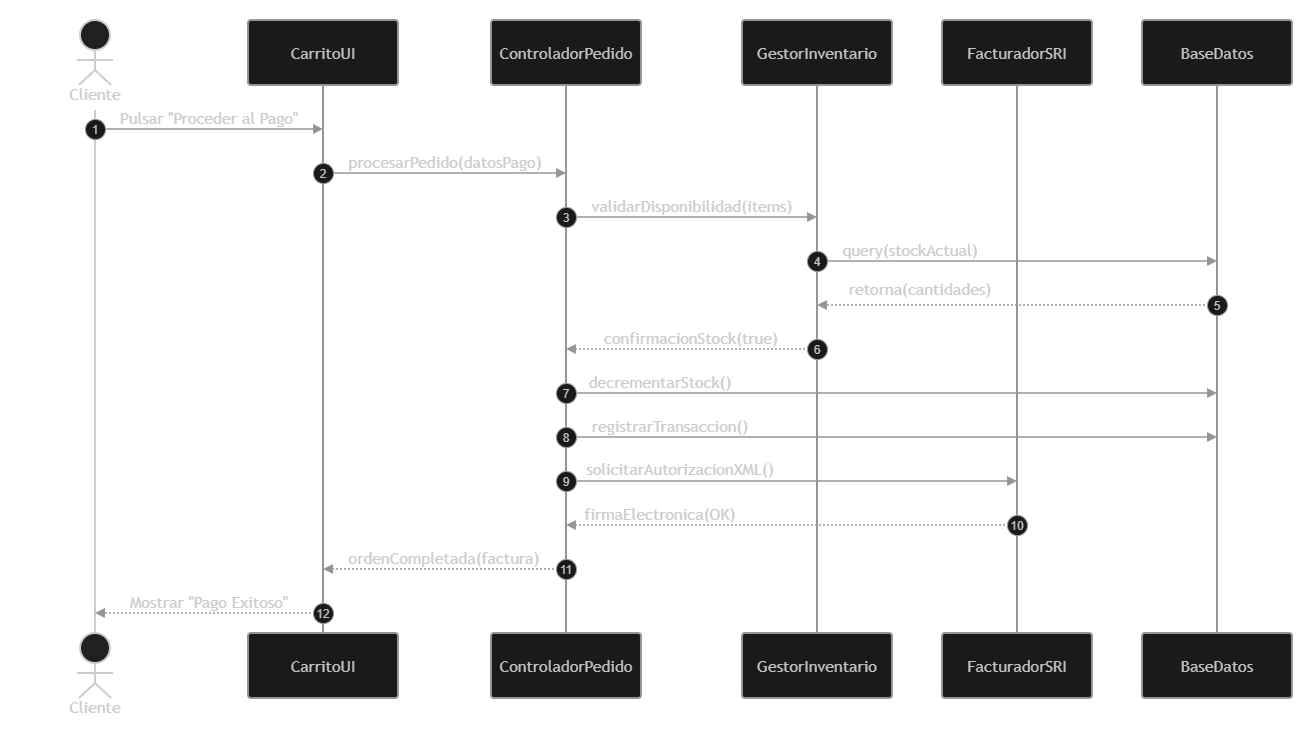
\includegraphics[width=0.60\textwidth]{Images/registroPedido.png}
    \caption{Diagrama de Secuencia - Registro de Pedido}
    \label{fig:secuencia_1}
\end{figure}

\begin{figure}[H]
    \centering
    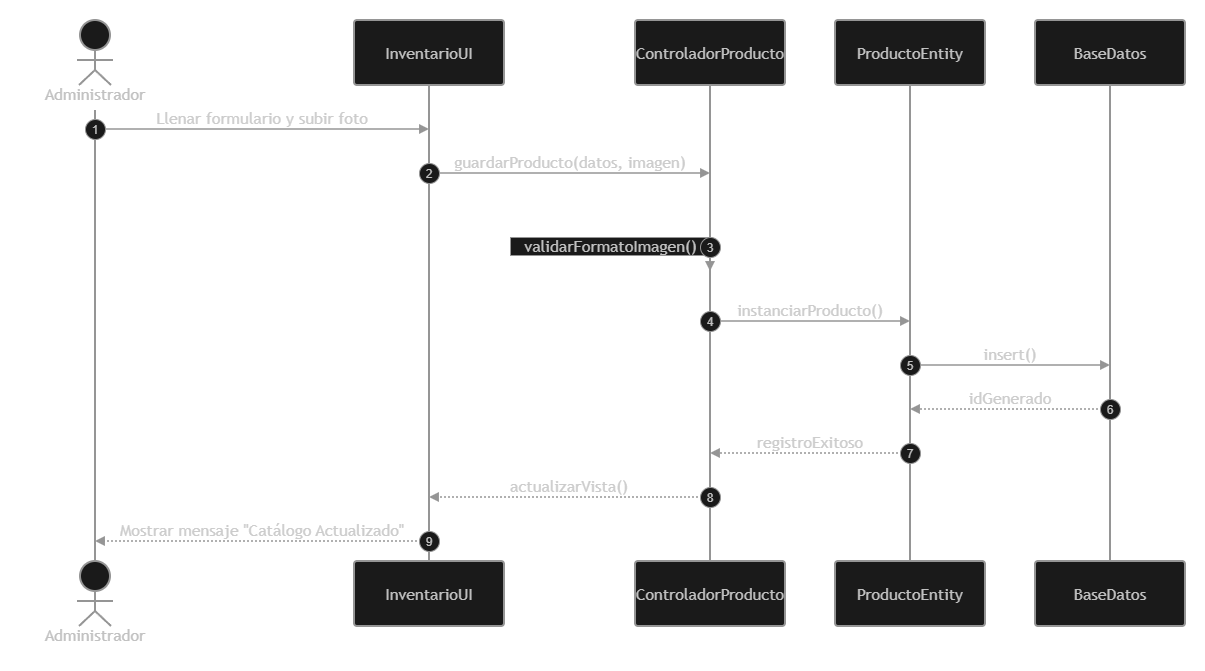
\includegraphics[width=0.60\textwidth]{Images/actuaizarCatalogo.drawio.png}
    \caption{Diagrama de Secuencia - Actualización de Catálogo}
    \label{fig:secuencia_2}
\end{figure}

\begin{figure}[H]
    \centering
    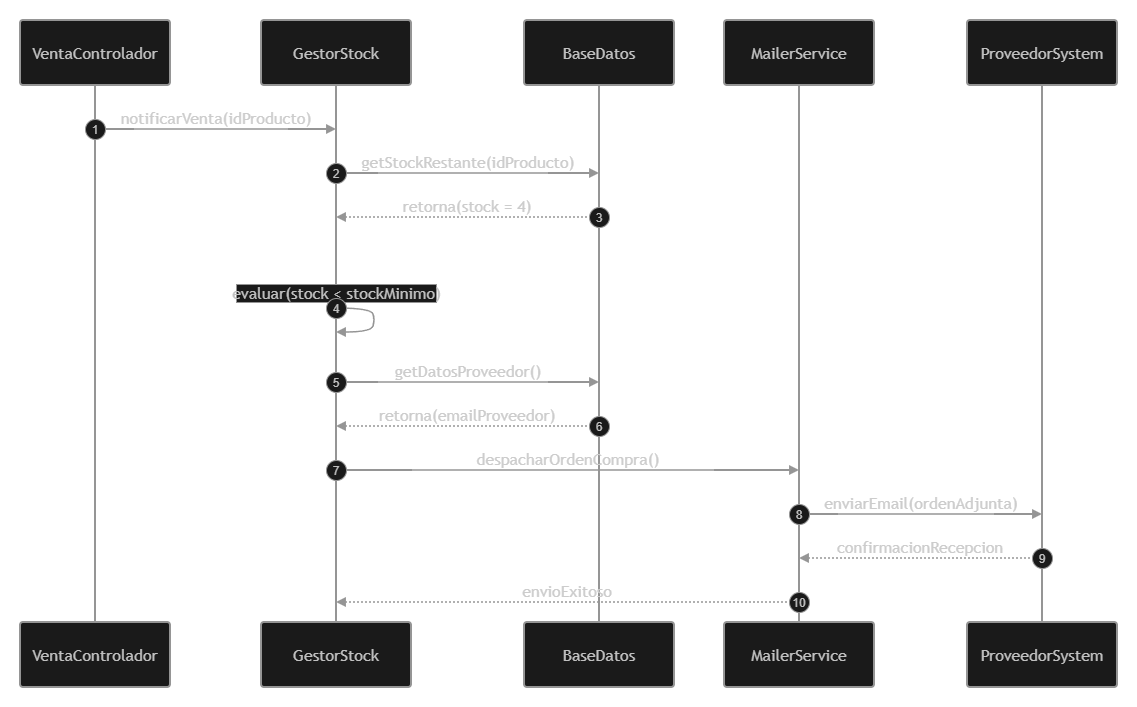
\includegraphics[width=0.60\textwidth]{Images/alertaRebastecimiento.png}
    \caption{Diagrama de Secuencia - Alerta de Reabastecimiento}
    \label{fig:secuencia_3}
\end{figure}

\subsection{Diagrama de actividades}
\begin{figure}[H]
    \centering
    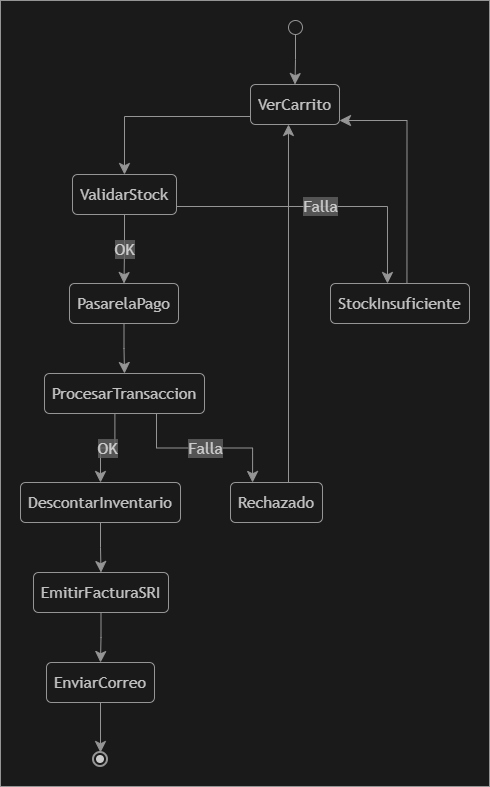
\includegraphics[width=0.60\textwidth]{Images/flujoCarrito.png}
    \caption{Diagrama de Actividades - Flujo de Compra y Pago}
    \label{fig:actividades_1}
\end{figure}

\begin{figure}[H]
    \centering
    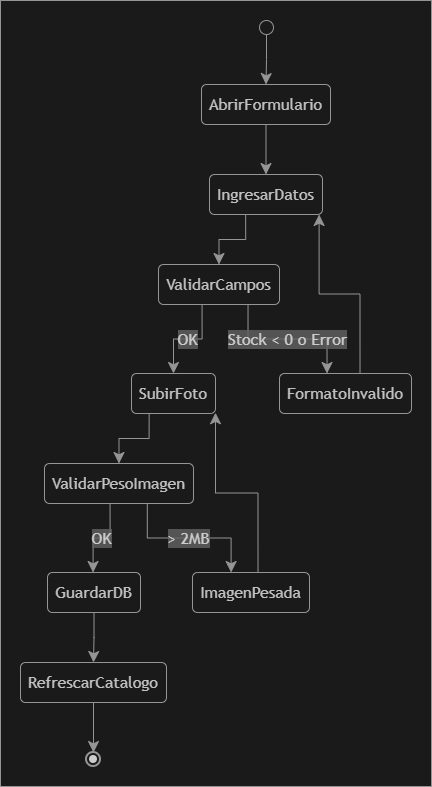
\includegraphics[width=0.60\textwidth]{Images/registroProductos.png}
    \caption{Diagrama de Actividades - Registro de Inventario}
    \label{fig:actividades_2}
\end{figure}

\begin{figure}[H]
    \centering
    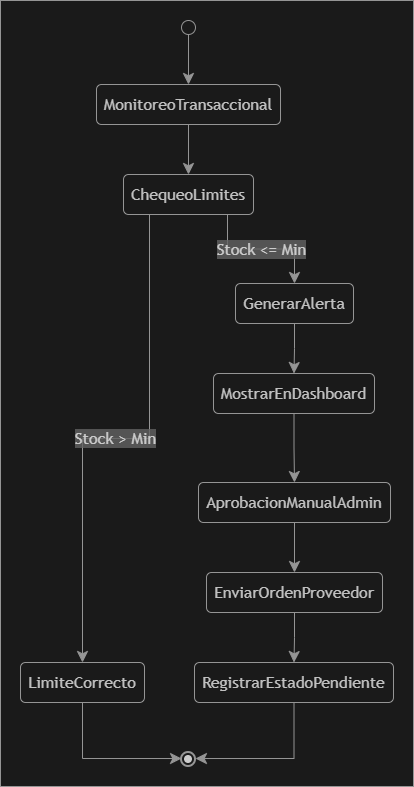
\includegraphics[width=0.60\textwidth]{Images/alertaRebastecimientoActividades.png}
    \caption{Diagrama de Actividades - Alerta de Reabastecimiento}
    \label{fig:actividades_3}
\end{figure}
\section{Diagramas estructurales}

\subsection{Diagrama de clases}
\begin{figure}[H]
    \centering
    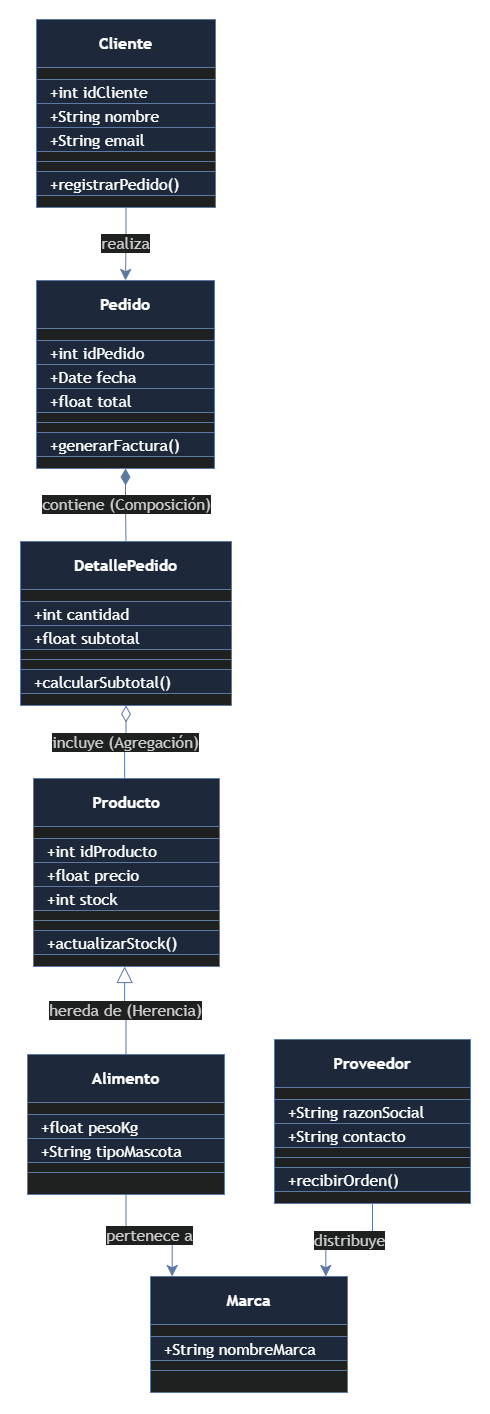
\includegraphics[width=0.50\textwidth]{Images/diagramaClases.png}
    \caption{Diagrama de Clases - Sistema de Comida de Mascotas}
    \label{fig:diagrama_clases}
\end{figure}

\subsection{Diagrama de despliegue}
\begin{figure}[H]
    \centering
    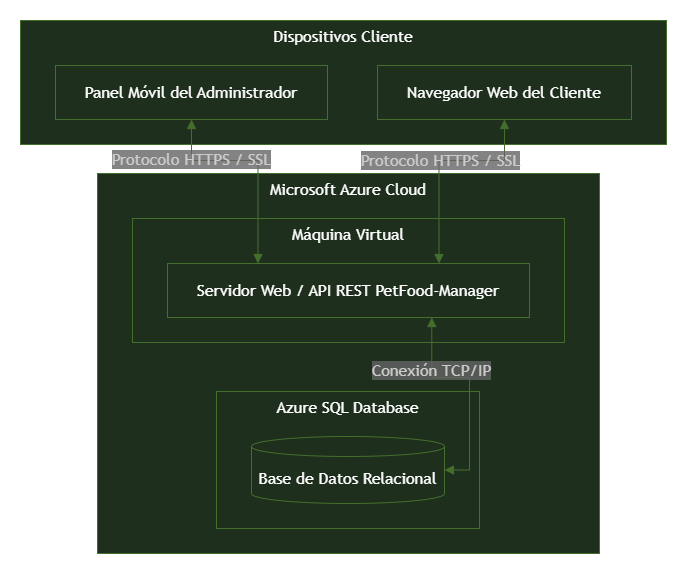
\includegraphics[width=0.60\textwidth]{Images/diagramaDespliegue.png}
    \caption{Diagrama de Despliegue de la Infraestructura Distribuida}
    \label{fig:diagrama_despliegue}
\end{figure}
\section{Solución informática}

\subsection{Mapa de navegación}
\begin{figure}[H]
    \centering
    \placeholderfig[5.5cm]{Mapa de Navegación del Portal de Alimentos de Mascotas (Administrador, Cliente, Visitante)}
    \caption{Mapa de Navegación de la Aplicación Web}
    \label{fig:mapa_navegacion}
\end{figure}

\subsection{Wireframe borrador del diseño de pantallas}
\begin{figure}[H]
    \centering
    \placeholderfig[5.5cm]{Wireframe Pantalla HOME (Catálogo de marcas de comida de mascotas, banner superior, footer)}
    \caption{Wireframe - Pantalla HOME}
    \label{fig:wf_home}
\end{figure}

\begin{figure}[H]
    \centering
    \placeholderfig[5.5cm]{Wireframe Pantalla LOGIN (Campos usuario, contraseña, validación)}
    \caption{Wireframe - Pantalla LOGIN}
    \label{fig:wf_login}
\end{figure}

\begin{figure}[H]
    \centering
    \placeholderfig[5.5cm]{Wireframe Panel de Administración (Gestión de stocks, catálogo, reportes de alertas)}
    \caption{Wireframe - Panel de Administración / Menú}
    \label{fig:wf_menu}
\end{figure}

\newpage
\subsection{Pantallas del proyecto terminado}
\begin{table}[H]
    \centering
    \small
    \renewcommand{\arraystretch}{1.5}
    \begin{tabularx}{\textwidth}{|p{5.5cm}|L|}
        \hline
        \rowcolor{upsblue} \textcolor{white}{\textbf{Nombre del caso de uso}} & \textcolor{white}{\textbf{Captura de Pantalla del sistema informático terminado}} \\
        \hline
        Registrar Pedido de Comida de Mascotas & 
        \placeholderfig[3cm]{Interfaz del sistema real en ejecución: Pantalla de carrito de compras, catálogo de alimentos y formulario de pago del cliente} \\
        \hline
        Actualizar Catálogo e Inventario de Alimentos & 
        \placeholderfig[3cm]{Interfaz del sistema real en ejecución: Panel administrativo agregando marca de comida y configuración de stock mínimo} \\
        \hline
        Emitir Orden de Reabastecimiento Automática & 
        \placeholderfig[3cm]{Interfaz del sistema real en ejecución: Dashboard de administración con alerta de stock crítico y la orden para el proveedor} \\
        \hline
    \end{tabularx}
    \caption{Evidencia de Pantallas del Sistema Terminado}
    \label{tab:pantallas_proyecto}
\end{table}

\subsection{Link del código fuente. Enlace de GITHUB}
La base de datos, código fuente y documentación del proyecto de comida de mascotas se encuentran en el siguiente repositorio:
\begin{center}
    \textbf{Repositorio en GitHub:} \url{https://github.com/XavierSig/petfood-manager-system}
\end{center}
\section{Conclusiones y Recomendaciones}
\begin{enumerate}
    \item \textbf{Conclusión 1 (Aplicación práctica - Modelado de Negocio):} \\
    El modelado del Modelo Contextual y el Diagrama de Flujo de Datos (DFD) de nivel 0 permitieron delimitar de forma precisa los límites de la aplicación ``PetFood-Manager'', logrando mapear y documentar los flujos de datos transaccionales de venta e inventario entre la tienda PetShop Huellitas \& Snacks y sus entidades externas (clientes, proveedores, SRI y pasarela de pago), eliminando la ineficiencia histórica del registro manual.
    
    \item \textbf{Conclusión 2 (Aplicación práctica - Gestión Estratégica):} \\
    La alineación directa de las funcionalidades del software con la estrategia de supervivencia MIN-MIN demostró ser vital para el impacto del negocio. El módulo de alertas y reabastecimiento automático ataca directamente el cuello de botella del control de existencias, disminuyendo costos de almacenamiento y permitiendo que una tienda mediana retenga su clientela y compita frente al retail masivo.
    
    \item \textbf{Conclusión 3 (Aplicación práctica - Casos de Uso y Requisitos):} \\
    El diseño minucioso de la especificación de casos de uso y la separación clara de los requerimientos funcionales y no funcionales estructuraron las bases del desarrollo. Definir los flujos excepcionales, como la desconexión con la pasarela de pagos o fallos del SRI, previno problemas futuros en producción, garantizando que el sistema cuente con políticas transaccionales robustas.
    
    \item \textbf{Conclusión 4 (Retos técnicos - Base de Datos Relacional):} \\
    Modelar el diagrama de clases e implementarlo bajo una base de datos relacional transaccional supuso el principal reto técnico en el diseño estructurado. Relacionar la herencia de los productos alimenticios según el animal destinatario junto a la composición obligatoria de las cabeceras de ventas con sus correspondientes detalles exigió aplicar restricciones de integridad referencial complejas para evitar redundancia e inconsistencias de datos.
    
    \item \textbf{Conclusión 5 (Retos técnicos - Arquitectura Distribuida):} \\
    Definir e integrar la arquitectura física del sistema sobre infraestructura distribuida de Microsoft Azure (máquinas virtuales para el servidor web y Azure SQL para la base de datos) demandó mitigar problemas de latencia de red y seguridad. Se solventó este desafío estableciendo conexiones cifradas SSL/TLS mediante protocolo HTTPS, asegurando la privacidad en el intercambio transaccional de pagos.
    
    \item \textbf{Conclusión 6 (Retos técnicos - Sincronización en Tiempo Real):} \\
    Garantizar la sincronización concurrente del inventario lógico y físico al procesar ventas masivas representó un reto de concurrencia avanzado. Fue necesario diseñar un flujo lógico donde las decrementaciones de stock se realicen de manera transaccional atómica, disparando eventos asíncronos para el envío de notificaciones automáticas al correo del proveedor, aislando los tiempos de espera del cliente final.
\end{enumerate}

\newpage
% 4. Generar la Bibliografía automáticamente desde bib.bib
\nocite{*}
\bibliographystyle{apalike}
\bibliography{bib}

\end{document}